%!TEX root = ../ArticleCalib_main.tex
%!TEX root = ../sections/articleCalib_section4_SinglePixResponse


%%%%%%%%%%%%% FIGURE 2 BERNOUILLI POISSON INTERVALLES


\begin{figure}[htbp]
\begin{center}
\captionsetup[subfigure]{position=top, labelfont=bf, textfont=normalfont, singlelinecheck=off, justification=raggedright }

\subfloat[]{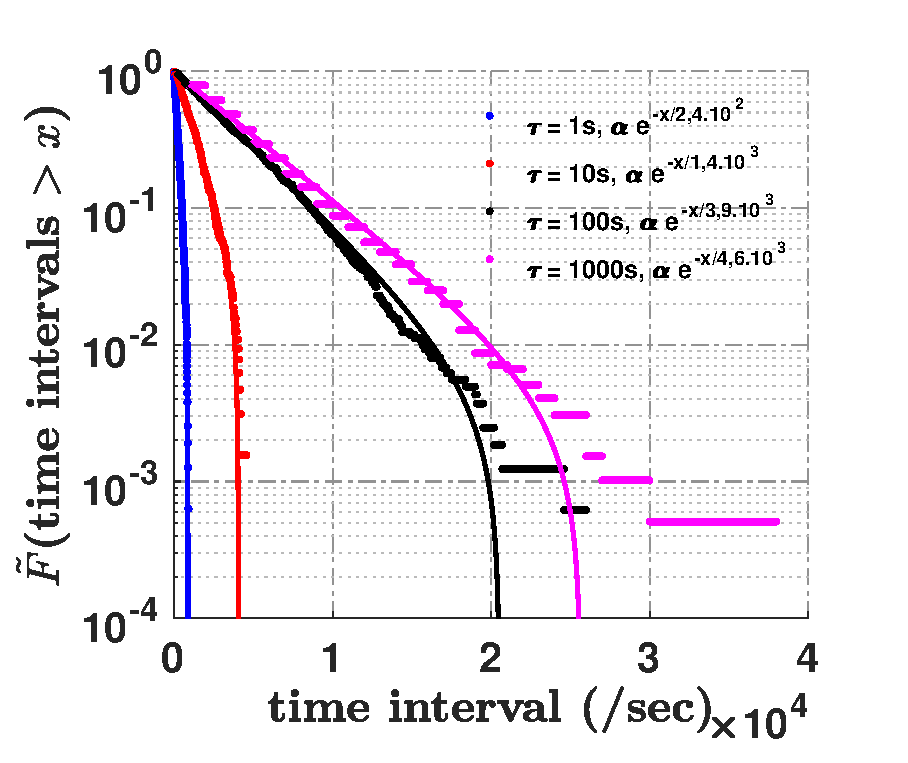
\includegraphics[width=0.4\linewidth]{fig2_ArgumentCompatiblesPoiss/fig2_Poiss_distriIntervalles.eps}\label{fig:PoissonsIntervals:A}}  
%\qquad
%\subfloat[]{\includegraphics[width=0.4\linewidth]{fig2_ArgumentCompatiblesPoiss/anlz_varmeanij_yxline_varexcess.eps}\label{fig:PoissonsIntervals:B}}  \\


\caption{{\bf Distribution of time intervals.} The complement of the cumulative distribution of the time intervals between two successive counts for a pixel$_{ij}$ for all pixels is represented. The time intervals are exctracted for differents times of exposure $\tau$ and fitted by an exponential model. For each $\tau$, the time constant found according to the model is given \subref{fig:PoissonsIntervals:A}} 
%{\bf All pixels are perfect Bernouilli.} The pixels can only take values 1 and 0. By definition they can be only fellow a  bernouilli law with  $\sigma_{ij_K}^2 = <$pixels$_{ij}>_K * (1-<$pixels$_{ij}>_K) $ strictly \subref{fig:PoissonsIntervals:B}. }

\label{fig:PoissonsIntervals}
\end{center}
\end{figure}
%%%%%%%%%%%%%%%%%%%

 	